\documentclass{article}

\usepackage{graphicx,color,tabularx,amsmath,amssymb,fancyvrb,soul}
\usepackage{subcaption}
\usepackage{float}

\title{CS310 Computer Science Project \\ Final Report \\ The Creation of an Android Application to Aid a Student's Revision of Edexcel GCSE Mathematics}
\author{Ryan O'Hara \\ u1702761}

\begin{document}

\maketitle

\newpage

\tableofcontents

\newpage

\section{Abstract}
\label{section:abstract}

\section{Introduction}
\label{section:introduction}

\subsection{Project Motivation}

This project was motivated by two key factors.

% Reference for studets thing: https://content.ebscohost.com/ContentServer.asp?EbscoContent=dGJyMMvl7ESeqLE4y9fwOLCmsEiep7NSsaa4SK6WxWXS&ContentCustomer=dGJyMPGntk60p65Juerwgd%2FiuY%2Fx1%2B6B&T=P&P=AN&S=R&D=ehh&K=53450186 (Accessed 23rd March 2020)
% Second reference: https://0-onlinelibrary-wiley-com.pugwash.lib.warwick.ac.uk/doi/pdf/10.1111/jcal.12184 (Accessed 23rd March 2020)

\subsection{Problem Outline}



\subsection{Project Specification}

This project aims to create an android application similar to MyMaths homework functionality. This will enable student's to load exam questions in a specific topic in Edexcel GCSE Mathematics and input an answer. This answer will then be compared to the original answer, and the student will get a visual response as to whether they answered the question correctly or incorrectly. Where the student answered the question incorrectly, the correct answer should be displayed to the student so they can compare their answer with the correct one. \\

To achieve this task a set of requirements were laid out during the project specification[x]. These requirements follow the MoSCoW system for writing requirements. The MoSCoW system groups requirements into four classes, must, should, could, and won't. All of the must requirements are vital to the success of the project, they need to be completed by the end of the project. At the completion of all of the must requirements, a minimum viable product (MVP) should be created. Should requirements are features which are not essential to the completion of a MVP but are features which are expected in the final product. Could requirements are features which are not expected in the final product, but if all other requirements are completed before the deadline, the could requirements will be implemented. Won't requirements are features which will not, under any circumstances, be present in the final product. \\

The requirements present in the project specification are as follows: \\

The Android application which will be created for this project must: 

\begin{enumerate}
	\item Have a start page with several clickable buttons
	\item Be able to run on Android devices with Android versions between Android 6 and Android 10
	\item Have a list of each module found in Edexcel's GCSE Mathematics Specification[10], with each module being selectable
	\item Generate revision questions where numerical values are generated by Java's inbuilt random number generator and make sense
	\item The user has the ability to input numerical answers to the revision questions generated (requires 4)
	\item When answers are submitted the user must receive feedback relating to whether	their answer matches the correct answer for the question, and where the user’s answer is incorrect, display the correct answer. \\
	
	The Android application which will be created for this project should:
	\item Have a variety of testing difficulties, ranging from easy to hard for each module
	\item Have a way of tracking user progress over a number of days or tests per module (requires 5)
	\item Display model methods for working out the correct answer for a question where the user inputted an incorrect answer (requires 6) \\
	
	The Android application which will be created for this project could:
	\item Include resources similar to those which would be used in a classroom environment to teach the user about a topic
\end{enumerate}

Project success was also defined in the project specification. To be deemed successful, the final product produced by this project will have completed: 

\begin{itemize}
	\item all of the must requirements defined above
	\item at least one of the should requirements defined above
	\item any value of could requirements defined above
\end{itemize}

The target audience for the final product of this project is students sitting Edexcel GCSE Mathematics examinations. The average age of students sitting this exam is 16 years old. Although, students as early as year 7 (age 11 - 12) begin learning content which is examinable in the GCSE Mathematics exam. The app will be primarily designed for 15-16 year olds, but needs to be accessible to students as young as 12. This means there are a group of non-functional requirements which were not outlined in the project specification but were followed during development which are shown below: 

\begin{itemize}
	\item The language used in the application should be understandable to 12 year old school children
	\item The application should be simple and minimalistic as to not confuse new users
	\item A 12 year old who has not previously used the application but is familiar with smartphones should be able to use the application effectively with minimal prompting
\end{itemize}

These functional requirements enable anyone learning the content for the Edexcel GCSE Mathematics exams to be able to use the application and benefit from it.


\subsection{Report Structure}

This report will start by running through the background to this project. The background section will outline the current landscape of the problem, what has currently been achieved by other people. It will be followed by an explanation of the software development methodology which was used throughout the development of this application. This methodology section will explain how the work was completed from a project management point of view, for example it will outline a typical development session. \\

Section \ref{section:design} outlines the design of the application which will provide a high level overview of the application. This high level view will explain the control and data flows of the program, and any specific design choices which was made throughout the development of this project. Section \ref{section:implementation} discusses the specific implementation details of the project. For example, how the questions were created in the application. Testing will be discussed in section \ref{section:testing}. This will consist of outlining how testing was conducted, and the results of user testing. \\

Then project management will be discussed in section \ref{section:projectManagement}. This section will be a discussion on several details of the project that cannot be seen from the source code, for example the development schedule, or weekly meetings with key stakeholders. These details do not appear in the source code but impact the project. The results section follows the project management section, where the requirements will be evaluated and the success of the project will be determined. \\

The conclusion will be section \ref{section:conclusion} which will summarise key findings in the report. This will be followed by the future work which could improve this project, and turn it from a proof of concept into an application which would be able to be released. Section \ref{section:issues} will discuss the legal, social, ethical, and environmental issues with this project. \\

The final section in this report will be the references. Harvard referencing style is adhered to throughout this report.\\ 

\section{Background}
\label{section:background}

There are two main GCSE Mathematics revision tools in use today that are used in schools. Both of the main revision tools are explained in depth in their respective sections. There are also a number of other independent revision tools which are not actively used in schools, but are able to be downloaded and used on mobile devices. 

\subsection{MyMaths}

The first tool is MyMaths[4] which is a website which aims to enrich a student's classroom learning experience. MyMaths main use case is to supplement the material covered in class by a teacher. The main feature of MyMaths is the online homework feature. This feature enables teachers to set homework to their class. This homework covers a specific topic, for example Venn diagrams, and the students can answer questions on this topic. Example homework questions on the topic of Venn diagrams can be viewed as figure \ref{figure:mymathsHomeworkQuestion1}.
\begin{figure}[H]
	\centering
	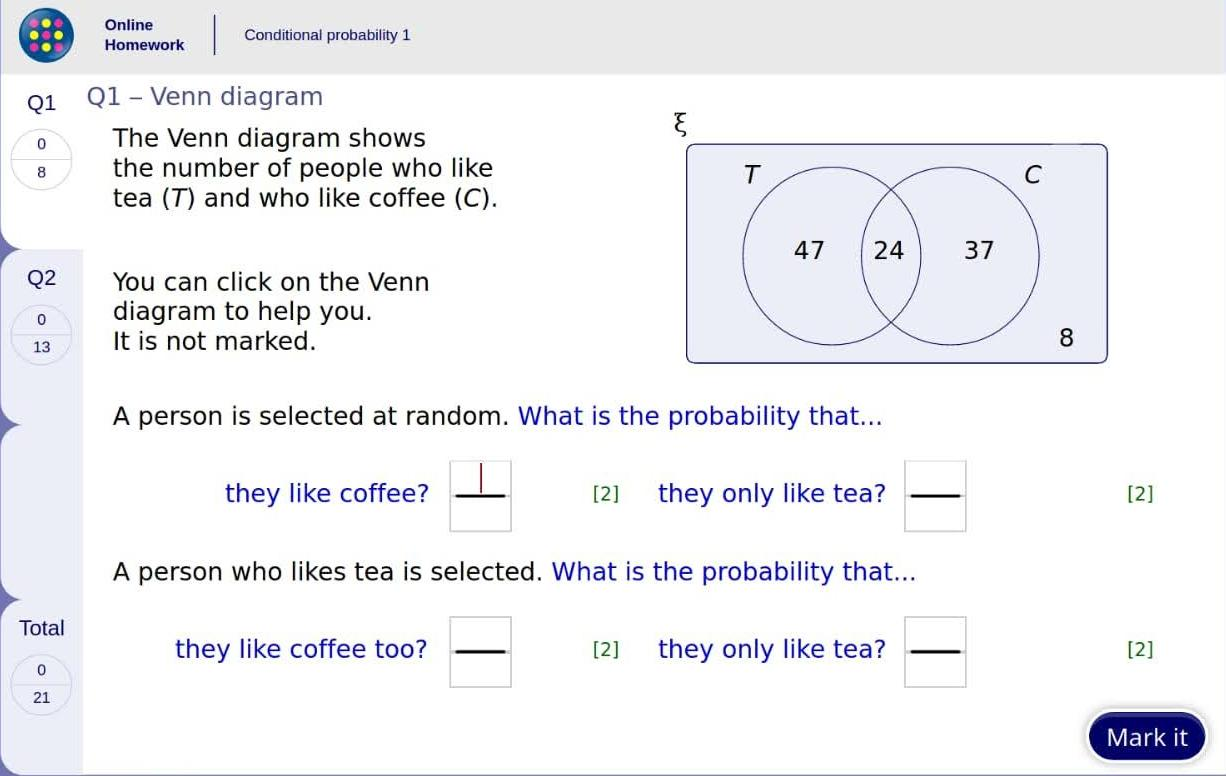
\includegraphics[width=0.9\linewidth]{./data/mymathsQuestion1.jpg}
	\caption{Venn diagram homework questions.}
	\label{figure:mymathsHomeworkQuestion1}
\end{figure}
The student's scores are then generated (as a percentage) and sent back to the teacher. \\

The values selected in the homework are unique each time a student attempts that specific homework. This prevents a student from memorizing a specific answer to pass the homework. A teacher can also see the number of attempts that a student has currently taken for the homework, and their highest score. Giving a teacher the ability to see the number of attempts that a student has at questions on a particular topic highlights where a student is struggling and can enable one on one teaching to boost the student's knowledge in that particular topic. A student can also attempt a homework which has not been set by their teacher. This allows a student to revise any topic in GCSE Mathematics on their own without a teacher. \\

MyMaths also gives a student the ability to take a lesson in any topic in GCSE Mathematics. This lesson walks through an example question in the topic, and then provides practice questions which are of a similar style to the homework questions. These questions are then marked, and where the student answers the question incorrectly, the correct answer is displayed next to the answer box. \\

MyMaths, however, is intended to be used in a web browser, and so is designed to be used on a desktop computer or a laptop. Due to the increase in smartphone adoption, more people of GCSE age have access to smartphones on a regular basis [x]. 
% find this figure somewhere
MyMaths has an iOS and Android application for tablets, but not a specific application for smartphones[5]. This prevents students who own their own smartphones but do not have access to a tablet on a regular basis from revising using MyMaths. \\

\subsection{Khan Academy}

The second main GCSE Mathematics revision tool is Khan Academy[6] which is a non-profit organization which aims to "provide a free, world-class education for anyone, anywhere"[6]. Khan Academy's main function is to teach new information to people. It does this through the use of short videos covering particular concepts. For example, there is a six minute video covering how to find a side of a triangle using the sine rule[7]. These videos aim to replace classroom teaching for those who are unable to attend school. There is a video for every topic in GCSE Mathematics and so a student could exclusively use Khan Academy to learn the content for their exams. Khan Academy also has a testing feature, where for a certain topic four questions come up which the user has to answer. This is, however, not available for all topics, and the user is limited to answering four questions at a time. \\

Khan Academy has applications in both major app stores, the Apple app store[8] and the Google play store[9]. This app runs on all major devices and has the same functionality as the website version of Khan Academy. Users can create accounts for free which keeps track of their progress and can access videos for all topics available on the website for free. \\

\subsection{Independent Revision Tools}

There are several other mathematics revision apps on both app stores, examples of which can be seen below as figure \ref{figure:appStoreApps}. These apps mostly focus on testing using some form of revision questions. These questions are either limited to multiple choice questions, or questions which have the same numbers each time they appear. This leads to two problems: random guessing for the multiple choice questions, or answer memorization for the questions which do not change their numbers. This leads to these applications not being endorsed in schools. \\

\begin{figure}[H]
	\centering
	\begin{subfigure}{0.8\textwidth}
		\frame{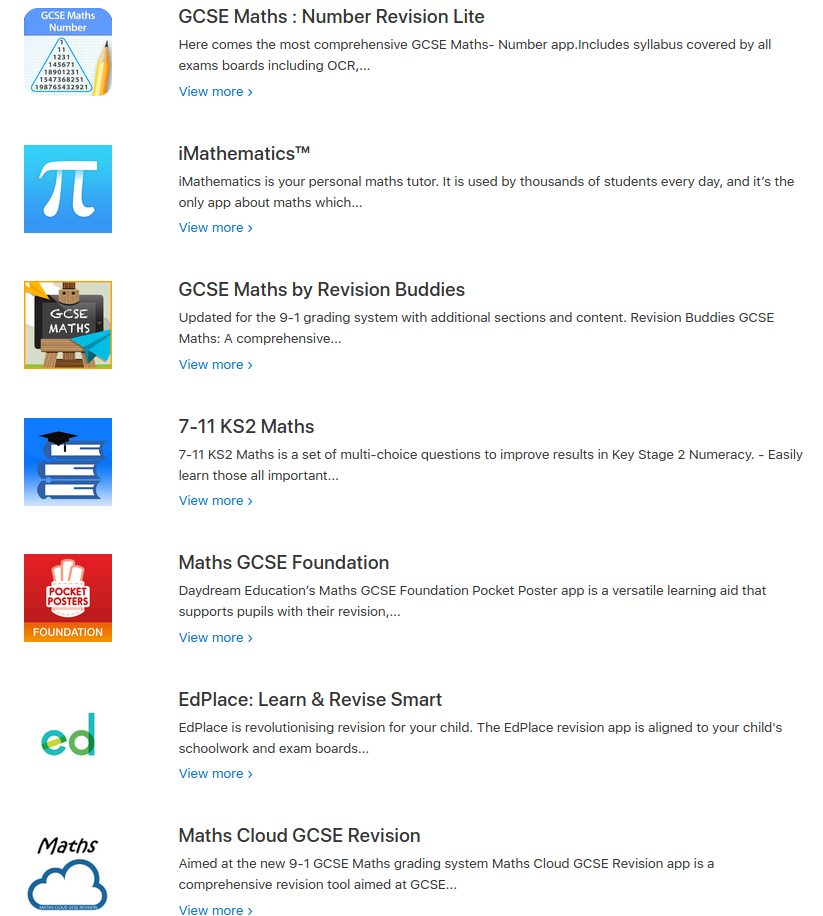
\includegraphics[width=0.9\linewidth]{./data/appleAppStoreApps.png}}
		\caption{Revision applications on Apple's app store}
	\end{subfigure}
	\hfill
	\begin{subfigure}{0.8\textwidth}
		\frame{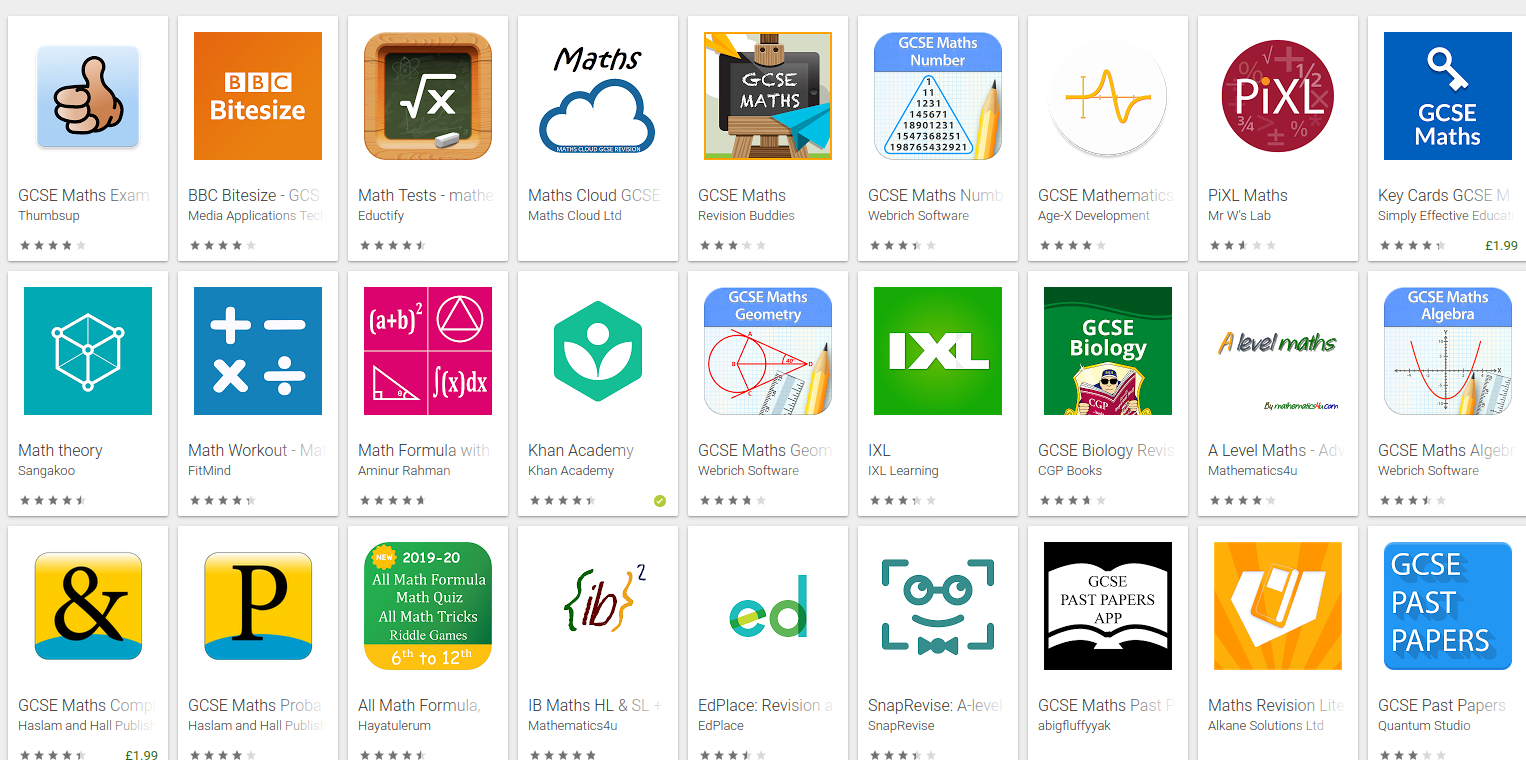
\includegraphics[width=0.9\linewidth]{./data/googlePlayStoreApps.png}}
		\caption{Revision applications on the Google Play store}
	\end{subfigure}
	\caption{Revision applications on both the Apple app store and the Google play store}
	\label{figure:appStoreApps}
\end{figure}

\subsection{Maths Watch}

Maths Watch[11] is an older tool which was used for teaching purposes in schools. This is a service which provides educational videos for students to learn from. It is designed to replace both classroom teaching and as a homework tool. Mathswatch is a subscription service, which only schools can subscribe to. If a student's school is not subscribed to Maths Watch then a student cannot get access to it. \\

Maths Watch has two main methods for distributing their video content. The first method is through DVDs which are posted to schools which buy them, and the students can then get these discs from the schools with all of the videos on them. The second method is through their online portal which provides the ability for paid users to stream video lessons. The Maths Watch service also states on the subscription page of their website[12] that they provide "A bank of 1000s of interactive exam-style questions for students' independent work with instant feedback". This is similar to MyMaths where a user can submit their answers and get feedback on whether they were correct, and if they were incorrect have the correct answer displayed. \\

The Maths Watch service is used by students all throughout the UK and is an incredibly valuable tool to aid their learning. Unfortunately, Maths Watch does not provide a mobile application on either of the major app stores (Apple iOS app store, or the Google Play store). As well as this, only schools can purchase Maths Watch, so if a students' school is not a Maths Watch partner, then the student cannot get access to Maths Watch. \\

\subsection{Gap in the market?}

A gap was spotted in the GCSE revision market, which consists of a mobile application which focussed on testing instead of teaching. It could be used alongside classroom learning, or other forms of learning which emulate the classroom environment, such as Khan Academy. This gap is what this project aims to fill, an application which focusses on testing skills already gained by the user from a classroom like environment, which will prepare the user for sitting their Edexcel GCSE Mathematics exam. \\

This application will have to provide users with the ability to practice skills gained from classroom learning. It must contain questions of GCSE exam standard so that students can effectively prepare for their exams using the application. 

%
%
%

\section{Methodology}
\label{section:methodology}

This project was conducted using an agile methodology. The project focussed on building a base product and then adding new features incrementally with each development cycle until the final product was produced. 

%Go into detail about the scrum methodology.

\section{Design}
\label{section:design}

This application had a target audience of school children between the ages of 12-16 years old. This meant that any design would have to be simple and intuitive to prevent users from getting 'lost' within the application. The graphs for both the control flow and the data flow for this application are acyclic as is shown by the two figures below, figure [y] and figure [z] respectively. Users can only follow certain paths, and will only end up in the same place by going backwards using the inbuilt backwards button in Android, so they cannot get confused about the layout of the application. Also, the number of pages was kept to a minimum for the application to function for the same reason. This minimalst design aims to prevent confusion by keeping the application simple to understand and use. \\

\subsection{Control Flow}

Figure \ref{figure:applicationControlFlow} is a graph for the control flow of the application. Each edge is bidirectional, the user can move forward by pressing a button in the application, and backwards by hitting the back button built into the Android operating system. \\

\begin{figure}[H]
	\centering
	\frame{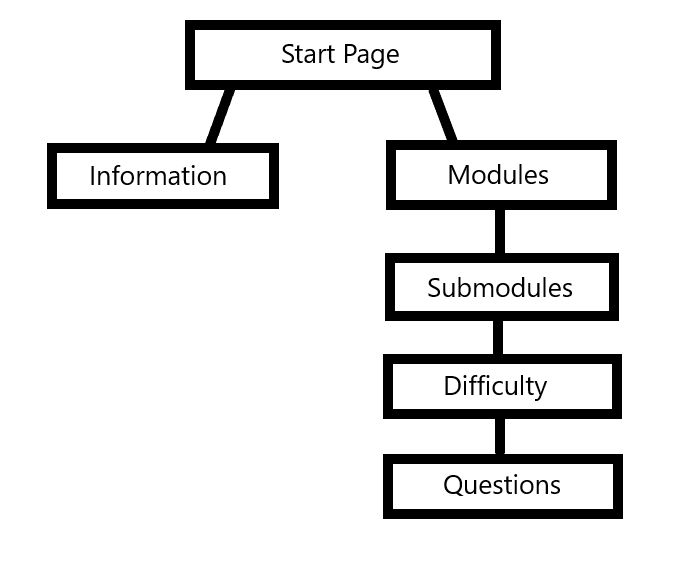
\includegraphics[width=0.9\linewidth]{./data/applicationControlFlow.png}}
	\caption{The control flow of the application.}
	\label{figure:applicationControlFlow}
\end{figure}

The only user choice in direction is at the start page where a user could select between the information page for the application and the modules list. The information page of the application just displays some basic information for the application. Each node in this graph represents an Android activity. An Android activity is the application equivalent to a webpage on a website. Activities are viewed as one screen in an application[15] and are intended to complete one specific task. If another task needs completing then the application should call another activity. Activities can contain fragments which can be thought of as "a modular section of an activity ... (sort of like a 'sub activity' that you can reuse in different activities)"[16]. The modules, submodules, and difficulty nodes in the control flow graph displayed above are activities which contain only list fragments. The list fragment class is a submodule of the fragment class which displays a list of items, and implements a listener which will act when the user clicks on a specific item. In the case of the modules node, the list displays all six modules which are examined in Edexcel GCSE mathematics. When the user clicks a specific module, the modules activity collects the information of the module selected, and starts the submodules activity and passes the information of the module selected onto the new activity. The submodules activity then displays the submodules for the module selected by the user. \\



% A control flow section is required in implementation to discuss how the modules node could be split into each of the six specific modules, and the submodules class could be split into each of the submodules depending on the module chosen. But it was decided to just have a modules class to make adding extra modules much more simple. 

\subsection{Data Flow}

Figure [x] is a graph of the flow of data throughout the application. When an activity starts another activity, it can pass information to it. This enables a single directional information flow throughout the application. That is why the diagram displayed as figure [x] is a directed graph. The direction of the data is denoted by an arrow, the side of the edge without the arrow is the sender of the data, and the side of the edge with an arrow is the data receiver. 

%\begin{figure}[H]
%\centering
%\includegraphics[width=0.9\linewidth]{./data/}
%\caption{}
%\label{figure:}
%\end{figure}

The data flow in this graph follows the minimalist design of this application. Data moves along a path in one direction so there is no confusion. A user can go back to a previous activity by using the inbuilt back button in Android. By doing this, the information selected further up the graph (closer to the root node) is preserved. This allows a user to utilise the back button to change the difficulty of the questions that they are answering while keeping the module and submodule information preserved. This enables simple use, where a user does not need to reselect all information to change one specific piece of data. \\

\subsection{Visual Design}

The visual design of this application is minimalist, in keeping with the rest of the app. Every page only has the necessary things displayed on it, and where applicable, only one thing displayed. Below are a few examples of this minimalist design. Figure \ref{figure:applicationStartPage} is a screenshot of the application's start page taken from the physical Google Pixel 2 device.

\begin{figure}[H]
	\centering
	\frame{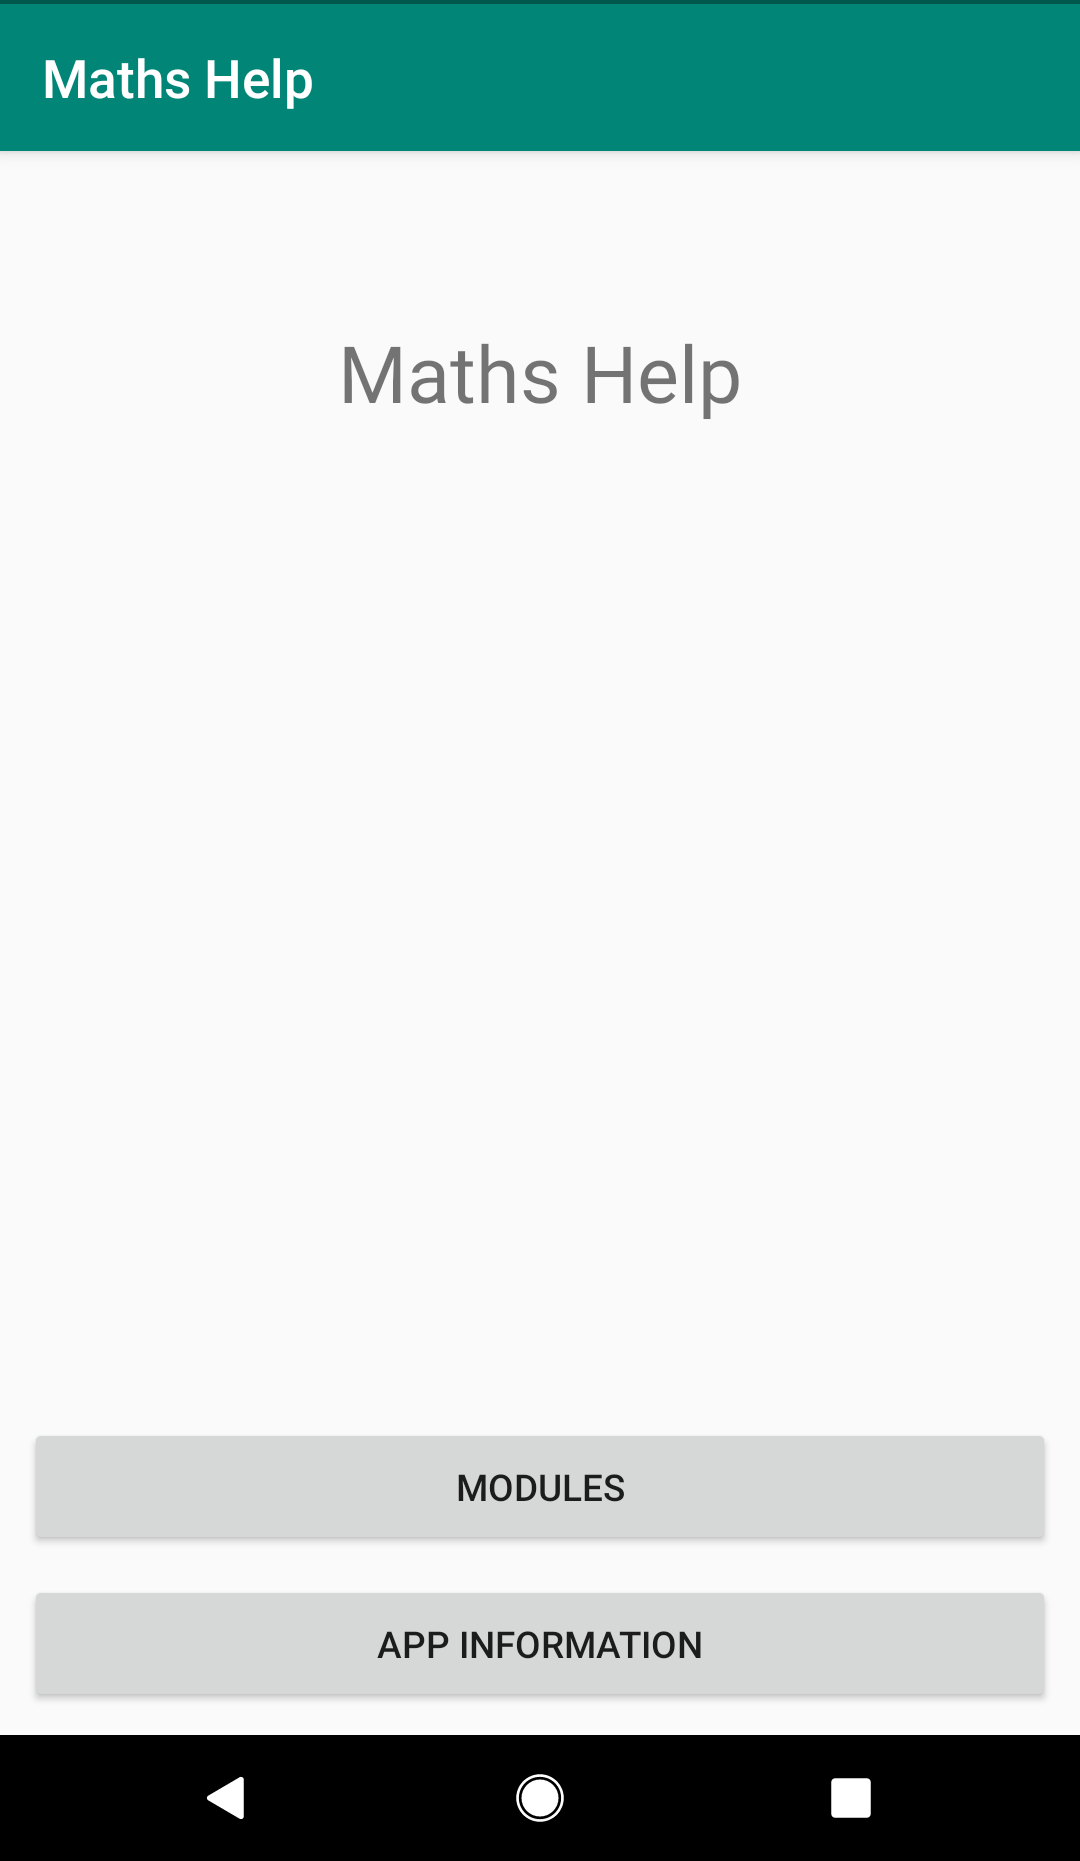
\includegraphics[width=0.9\linewidth]{./data/applicationStartPage.png}}
	\caption{}
	\label{figure:applicationStartPage}
\end{figure}

This screen is made up of the least amount of distinct elements that is possible. As it is the start page of the application it has to have the application name displayed, which is the Maths Help text at the top of the screen. The bottom of the screen is dominated by two buttons, one which starts the modules activity (the modules button), and one which starts the information activity (the app information button). There is nothing else on the webpage, and this is the least amount of elements with which to follow the control and data flow graphs displayed above. \\

An example of list fragment pages is the modules activity page. This is displayed below as figure \ref{figure:applicationModulesPage}, also taken from the physical Pixel 2 testing device. 

\begin{figure}[H]
	\centering
	\frame{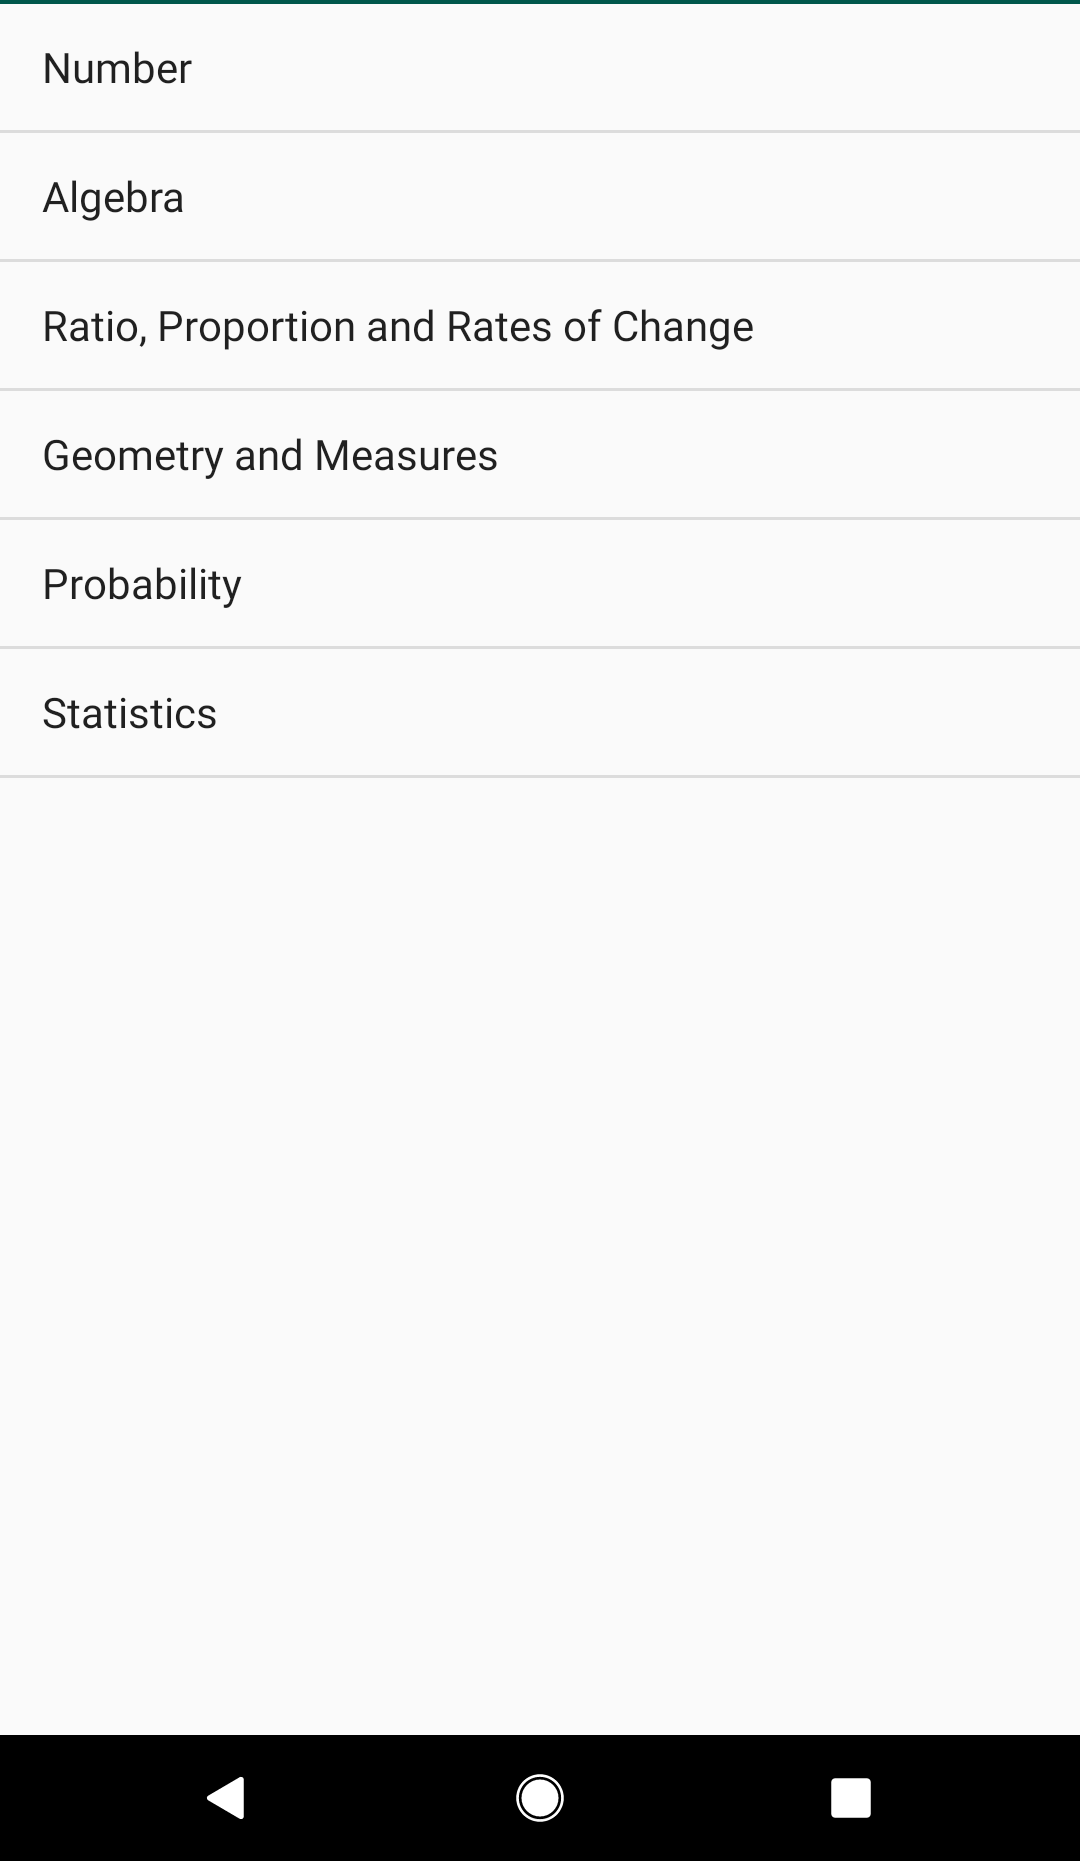
\includegraphics[width=0.9\linewidth]{./data/applicationModulesPage.png}}
	\caption{The modules activity page.}
	\label{figure:applicationModulesPage}
\end{figure}

% Discuss the control flow of the program, why it works the way it does etc...
% Get the control flow diagram from the presentation and discuss how pages are connected
% Make a new diagram, a more impressive one, which also shows the information transfer between the 
% separate activities.

\section{Implementation}
\label{section:implementation}

%
%

\subsection{Questions}

%
%

\section{Testing}
\label{section:testing}

The project specification[x] stated that this project would "implement test driven development". The progress report[x] described that test driven development would not be used as the testing method for this project, and that user testing would be used throughout this project. \\

The decision to change from unit testing to user testing was made because this project creates a tangible product in the form of an Android application. Writing unit tests for an android application was deemed to be time wasted, as this time could be spent writing other code. An android application is judged by users for unquantifiable reasons, such as the "feel" of the application. This can only be tested by a person using the application, and since this determines how satisfied a user is with the application testing for the unquantifiable qualities of an application was prioritised over unit testing. \\

\subsection{Testing Methodology}

All application testing was conducted on a physical Google Pixel 2 device, as well as at least one emulated virtual device. The emulation software used is the emulation software built into the Android Studio IDE. The emulator is called Android Virtual Device and [13]"The emulator provides almost all of the capabilities of a real Android device". The emulator provides an environment to test the application on a variety of devices with different capabilities to test that it works on the majority of Android devices. The application was tested on three virtual devices: 

\begin{itemize}
	\item HTC Nexus One (Smartphone)
	\item HTC Nexus 10 (Tablet)
	\item Google Pixel 3 (Smartphone)
\end{itemize}

These devices give a good variety in Android devices, between both tablet and smartphone, and old and new. These devices were chosen because if the application works well on all four devices, the physical Google Pixel 2 as well as the three virtual devices, then the application was likely to work on most Android devices. \\

Two types of user testing were conducted throughout this project, white box testing and black box testing. \\ 

\subsubsection{White Box Testing}

White box testing was conducted after each sprint cycle, where the developer would download the application onto their physical pixel 2 testing device as well as the range of virtual devices mentioned above, and then test that the application compiled and ran without errors. Other small tests were also conducted when testing new features. An example of this feature test would consist of the developer creating expected states of the application given specific inputs, and then the developer would follow the input sequence on all four testing devices, and ensure that the application ended up in the expected state for each device. Visual tests were also conducted, where an activity (which can be imagined as the application equivalent of a webpage in a website) in the application was drawn on paper, and then loaded up in the application for each of the testing devices, and the layout on the testing devices was compared with the layout drawn on paper. This testing method was used to find visual errors in the application. \\

\subsubsection{Black Box Testing}

Black box testing was conducted using users outside of the development team. These users were not shown the source code for the application, and this testing was conducted primarily on the physical Pixel 2 testing device. The user would be provided with the application and their use of it would be observed. Before any testing was conducted verbal consent was gained from the user for testing the application through observing their use case. If it was the first time the user had used the application then they were asked to try to use the application as if they had just downloaded it from their normal app store. Whereas, if a user was familiar with the application then they were asked to complete a task which utilised a new feature, or asked to compare visual styles with an image of both the current and previous styles, although the user was not made aware of which style was the current application style, and which was the previous application style. Where there was a change in a feature that the user had used before, they were not notified of the change, and how they dealt with the change was noted. \\

Black box testing was conducted after every major feature was added, with the results being used to improve the feature. Users of different mathematical ability were asked to test the application, from colleagues who use mathematics every day in their fields of study, to those who last encountered it when they took their GCSEs. White box testing was conducted throughout development. This was because compilation tests were quick and easy to conduct, taking around one minute per test and requiring access to the physical testing device, and would display errors in the code which would then be fixed before attempting the compilation test again. \\

%
%
%

\section{Project Management}
\label{section:projectManagement}

This project was a large software engineering project, especially for a team size of one. This meant that effective project management was required to keep the project going and make it a success. 

\subsection{Schedule}

A schedule was created early, and updated throughout the project to represent and handle the amount of work which had been completed. Two key versions of the schedule were displayed to various stakeholders throughout the project in key documents. These key documents were the project specification and the progress report. 

\subsubsection{Project Specification Schedule}

At the beginning of this project a schedule was created. This schedule aimed to complete all of the requirements stated in the project specification[x] by the end of the project. The schedule was created using a technique common in industry which involved some numbered cards. Each requirement was reviewed with each review consisting of analysing the relative difficulty of the requirement with respect to all the other requirements. The difficulty was quantified using the numbered cards, the cards would follow a logarithmic pattern, doubling with difficulty each time. The lowest valued card was \textsuperscript{1}/\textsubscript{4} and the largest value was 16. Any requirement with a relative difficulty value greater than 16 was then broken down into sub-requirements and these sub-requirements would then be reviewed, and broken down further if their relative value was also above 16. \\

This relative difficulty in requirements was used to create a rough schedule for the project. The schedule created for the project specification can be seen as a Gantt chart in figure \ref{figure:projectSpecGanttChart}. \\

\begin{figure}[H]
	\centering
	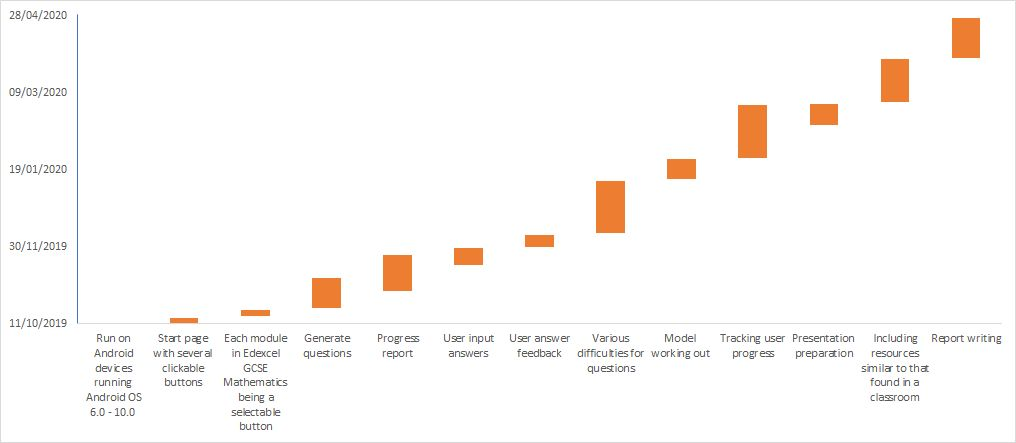
\includegraphics[width=\linewidth]{./data/projectSpecGanttChart.png}
	\caption{Gantt chart of the schedule produced for the project specification.}
	\label{figure:projectSpecGanttChart}
\end{figure}

This schedule was an optimistic schedule. It assumed all of the requirements would be completed by the end of the project, whereas the project specification's definition of success did not need all requirements to be completed. 

%
%
%

\subsubsection{Progress Report Schedule}

The progress report submitted on 24\textsuperscript{th} November 2019 updated this schedule, once it was realised that development was slower than initially intended through term one of this academic year (October 2019 - December 2019) due to personal reasons. The new schedule, referred to from now on as the Christmas schedule, again made the assumption that every requirement would be completed before the deadline. To mitigate against the slow development conducted through term one, the Christmas schedule increased the workload of the project throughout the Christmas period (8\textsuperscript{th} December 2019 - 8\textsuperscript{th} January 2020) and throughout term two of the project. \\

A Gantt chart created for this updated schedule can be viewed below as figure \ref{figure:progressReportGanttChart}

\begin{figure}[H]
	\centering
	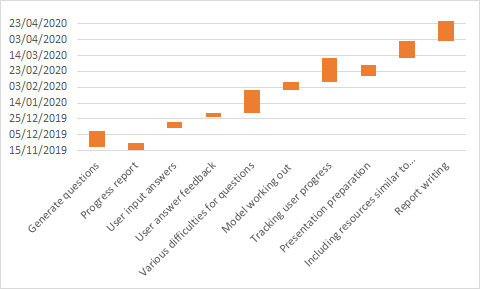
\includegraphics[width=0.9\linewidth]{./data/progressReportGanttChart.png}
	\caption{Gantt chart of the updated schedule produced for the project specification.}
	\label{figure:progressReportGanttChart}
\end{figure}

%
%
%

\subsubsection{Schedule Evaluation}

The image displayed below as figure [x] is an assessment of the completion of the final requirements in respect to the project specification schedule. 

%
%
%

\subsection{Tools}

This project utilized several tools to aid in the development of this Android application. Two of the main tools used to add value to this project are outlined below, one from a development point of view and one from a project management standpoint. 

\subsubsection{Android Studio}

Android Studio was used as an IDE (Integrated Development Environment) throughout development as it comes with many useful built in features. These features are specifically designed with android app development in mind. Examples of these features are: 

\begin{itemize}
	\item Rendering engine which converts XML into how it will appear in the application itself
	\item Android phone emulator
\end{itemize}

The rendering engine enables both the ability to edit the XML tags and see the effects in real time, as well as the ability to edit directly into the rendering engine with a drag and drop feature. This enables quick prototyping for new pages through the use of the drag and drop feature whilst also allowing a much larger degree of control through the ability to directly edit the XML.\\

Use of the android phone emulator enabled quick and efficient testing cycles. When a feature was initially developed, it could be tested on a wide range of devices through the phone emulator. This add on enabled the emulation of any modern phone through the ability to download files specific to that device. The app could then be tested on an accurate test bed, seeing how the app would look and work on a mobile device. Tablets could also be emulated, which helped with ensuring the application worked on a wide variety of devices.\\

The Android Studio IDE greatly increased the efficiency of development. This was encouraged through the notion that it was only designed specifically for android development, and so could focus entirely on that. Being built upon the IntelliJ platform meant that code editing was smooth and intuitive. \\

\subsubsection{Git}

Git was used as version control for this project. This enabled access to the project from any device, anywhere, anytime. It also enabled the ability to revert back to an earlier version of the project if something went wrong. This meant that development could take place without fear of failure, as if anything went wrong the project could just be reverted to the last working state.\\

The repository for this project can be found at the link in reference [14]. This repository is public and can be accessed by anyone. This enables anyone to see the code that would be running on their machines.\\

Git also logs the time when a change is made to the code. This enabled precise tracking of requirement completion and aided project management. Git commit messages for this project were all deliberately helpful. Git commit messages were written so that they would explain the changes made to the codebase, so they could be logs of when project requirements were completed. The git commit messages for this project can be viewed and give a detailed timeline of when requirements were completed and features were added. This was incredibly useful as it gave updates of any changes made to the codebase as soon as it was available to anyone who follows the repository, and also was used to create a timeline of when requirements were completed for this final report. \\

% Move into the methodology section. Certainly the information about the notes file.
\subsection{Weekly Work????}

Weekly meetings were held with the project supervisor to keep key stakeholders in the project up to date with development. Alongside weekly meetings, access was given to the project supervisor to the  github repository early in development. This enabled the project supervisor to directly monitor completed work. \\

A document in the github repository called notes.txt is a file which was edited after every development session was completed. This file contained notes on what was intended to be completed during each development session, as well as what was actually completed. A substantial amount of time was spent at the beginning of early development sessions on remembering what had been completed throughout the previous development session, what state the code was in, and what needed to be completed in this development session. This file cut down the time spent at the beginning of development sessions looking through previous git commits, and so overall this file caused development to be more efficient. \\

% \subsection{Project Management Evaluation} [Maybe don't include this]

% Use analysis from project management to assess the overall management of the project


\section{Results}
\label{section:results}

This section will evaluate the final application produced by this project and compare it against the requirements and definition of success set out at the beginning of this report. 

\subsection{Requirements}

The final application satisfies all of the must requirements. This means that the final application can display a question for users to answer, have an input field accepting numerical values, and when an answer is submitted, compare it to the pre-calculated answer and display whether the two answers match. If the two answers are different, then the correct answer is displayed for the user to see. \\

One of the three should requirements for this project was completed outright. Requirement 7 was changed between the progress report and the project presentation. It was changed from "Have a variety of testing difficulties, ranging from easy to hard for each module" to "Have two separate testing difficulties, foundation and higher, for each module". This change was made as the Edexcel GCSE Mathematics exams are split into two categories, of foundation and higher. The foundation tier of exams range from grades 1-5 and the higher range from grades 4-9, with the higher tier covering all content in the foundation tier and build on it. As this tier system already existed, and changing to easy, medium, and hard would only confuse students, the decision to switch to Edexcel's system was made. \\

Requirements 8 and 9 were not completed but are in progress. These requirements have been started and prototypes for each requirements have been made. Model working out has been created for three different questions in the algebra topic. These model working out are displayed when the user submits an incorrect answer. \\

The could requirement has not been completed. This is because requirements 8 and 9 have not been completed so work for requirement 10 has not been started. \\

As non-functional requirements are difficult to test, it is difficult to determine in absolutes whether these requirements have been met. Any tests conducted with 12 year olds to determine their comprehension of the questions in the application would not have been representative of the population as a whole, this method was not used to attempt to assess the completion of the non-functional requirements. Instead, user testing was conducted with colleagues who work with students of GCSE age range. Their feedback was incorporated into the development process as explained in the testing section of this report. Their feedback on the final application was that the functional requirements have been completed for almost all students who are in the English year 11, and the majority of students in the English year 9. Because of this, these functional requirements have been deemed completed for this project. \\

\subsection{Results Overview}

% This project could have been more impressive if it had been managed better
% But overall the project was of good quality and did what it had set out to do	

\section{Conclusion}
\label{section:conclusion}

\section{Future Work}
\label{section:futureWork}

\section{Legal, Social, Ethical, and Environmental Issues}
\label{section:issues}

This project did not face many legal, social, ethical, or environmental issues as it was a safe topic. There were no environmental or social issues faced for this project. There were limited legal and ethical issues which will be discussed under their respective subheadings. 

\subsection{Legal Issues}

There was one legal issue faced throughout this project. This issue was related to the tools which were used. As the final source code was not all written by the development team for this project; some of the code was generated through the tools used to aid this project, for example any code pre-generated through the Android Studio IDE was included in the final source code. This could create legal issues due to copyright laws. \\

This is why the licensing for all the tools used is linked below as a reference, and relevant sections are quoted to ensure that there are no legal issues with this project. \\

\subsubsection{Android Studio}

Android Studio is built on top of the IntelliJ platform. It shares the same license as IntelliJ, as is shown in this comment on a blog post by the creator of IntelliJ Dmitry Jemerov (Yole in the blog post) [17]. The IntelliJ IDEA (the IntelliJ IDE) is licensed under two licenses, but as is explained in the blog post, the licensed version of IntelliJ IDEA that is used as the basis of Android Studio has the Apache 2 license. The relevant sections of the Apache 2 license are as follows: "You may reproduce and distribute copies of the Work or Derivative Works thereof in any medium, with or without modifications, and in Source or Object form"[19]. This allows for the use of the IntelliJ and Android Studio IDEs for commercial and independent development which this project falls under, and so there are no legal issues with using Android Studio as the IDE for this project. \\

% Find the licensing for Android Studio, the link which proves that it copies the IntelliJ license, and then the 
% relevant parts of that license. 

\subsubsection{Git}

The majority of git is released under the GNU public license [2] which enables copying, modifying, or distributing git under any circumstances. The relevant sections of the GNU licence (from the preamble): "By contrast, the GNU General Public License is intended to guarantee your freedom to share and change free software--to make sure the software is free for all its users.". This enables free use of git for this project. \\

Small sections of git are not licensed under the GNU public license, but under the GPL (GNU Lesser Public License) [3]. Relevant sections from the GPL preamble: "By contrast, the GNU General Public Licenses are intended to guarantee your freedom to share and change free software--to make sure the software is free for all its users.". This enables the free use of git for this project. \\

As these are the only two external tools used throughout this project, and the only tools which could have impact on the source code of this project, then there are no legal issues with this project. Any other materials were produced by the author specifically for this project, and so there are no legal problems with using these materials. \\

\subsection{Ethical Issues}

This project only contains one key ethical issue, which is to do with the testing of the final product. Testing was conducted on colleagues who gave verbal and written consent to test the application. User testing was conducted where the user was observed using the application. This testing method makes this project one which does not require ethical review under department guidelines which can be found here [1]. "Student projects with primarily an educational purpose, for example asking peers or family members to test software as part of your course. Such projects should not include any form of deception or coercion or involve vulnerable groups (e.g. schoolchildren)." As testing was not conducted on school children for this project, instead user testing was conducted on colleagues over the age of 18, this project is ethically sound. 

\section{References}
\label{section:references}

[1] - https://warwick.ac.uk/fac/sci/dcs/teaching/ethics (Accessed 22\textsuperscript{th} March 2020) \\ 

[2] - https://github.com/git/git/blob/master/COPYING (Accessed 22\textsuperscript{th} March 2020) \\ 

[3] - https://github.com/git/git/blob/master/LGPL-2.1 (Accessed 22\textsuperscript{th} March 2020) \\  2020)

[4] - https://www.mymaths.co.uk/ (Accessed 22\textsuperscript{th} March 2020) \\ 

[5] - https://www.mymaths.co.uk/help.html (Accessed 22\textsuperscript{th} March 2020) \\

[6] - https://www.khanacademy.org/ (Accessed 22\textsuperscript{th} March 2020) \\

[7] - https://www.khanacademy.org/math/trigonometry/trig-with-general-triangles/law-of-sines/v/law-of-sines (Accessed 22\textsuperscript{th} March 2020) \\

[8] - https://apps.apple.com/gb/app/khan-academy/id469863705 (Accessed 22\textsuperscript{th} March 2020) \\ 

[9] - https://play.google.com/store/apps/details?id=org.khanacademy.android (Accessed 22\textsuperscript{th} March 2020) \\

[10] - https://qualifications.pearson.com/content/dam/pdf/GCSE/mathematics/2015/specification-and-sample-assesment/gcse-maths-2015-specification.pdf (Accessed: 6 October 2019) \\

[11] - https://mathswatch.co.uk/ (Accessed 25\textsuperscript{th} March 2020) \\

[12] - http://www.mathswatch.co.uk/subscription/4594745491 (Accessed 25\textsuperscript{th} March 2020) \\

[13] - https://developer.android.com/studio/run/emulator (Accessed 26\textsuperscript{th} March 2020) \\

[14] - https://github.com/AlphaMustang/thirdYearProject (Accessed 28\textsuperscript{th} March 2020) \\

[15] - https://developer.android.com/guide/components/activities/intro-activities (Accessed 28\textsuperscript{th} March 2020) \\

[16] - https://developer.android.com/guide/components/fragments (Accessed 28\textsuperscript{th} March 2020) \\

[17] - https://blog.jetbrains.com/idea/2013/05/intellij-idea-and-android-studio-faq/\#comment-4939 (Accessed 29\textsuperscript{th} March 2020) \\

[18] - https://www.jetbrains.com/idea/features/ (Accessed 29\textsuperscript{th} March 2020) \\ 

[19] - https://www.apache.org/licenses/LICENSE-2.0 (Accessed 29\textsuperscript{th} March 2020)

\end{document}